\part*{CyaVision}

Ce Module permet de surveiller un groupe de machines. En effectuant une batterie de tests à intervalles périodiques sur plusieurs serveurs. Et traite les résultats avant de renvoyer par mails les différentes erreurs.

\section*{Structure}

L'application est composée de 3 classes ayant des tâches bien déterminés

\begin{itemize}
	\item \textbf{Config} : son rôle est de récupérer et de traiter la configuration en base de données et si celle-ci est correcte, la mettre en forme avant de la transmettre à l'application principale. 
	\item \textbf{Supervisor} : est l'interface publique de l'application, elle permet de lancer les tests désirés.
	\item \textbf{Treatment} : traite les résultats provenant de la classe Supervisor et en cas de problèmes, envoie un mail soit au sysadmin soit à la personne responsable du projet posant problème. 
\end{itemize}

\begin{figure}[h!]
	\centering
	\includegraphics[scale=0.5]{images/UML_supervision_v2.png}
	\caption{Diagramme de classe de l'application}
\end{figure}

Ce package intègre aussi différentes classes de tests déjà existantes qui réalise les opérations sur les serveurs:

\begin{itemize}
	\item \textbf{MySQL} : comme son nom l'indique cette classe réalise des tests sur les serveurs MySQL, le plus généralement sur port 3306.
	\item \textbf{PyLobby} : celui-ci permet d'effectuer des tests sur n'importe quel port et donc n'importe quel protocole.
	\item \textbf{Relay} : permet d'opérer sur un protocole interne 
\end{itemize}

\underline{Remarque}:

Pour l'instant l'intérêt de ces différentes classe n'est pas évident car la classe PyLobby peut tout à fait remplir le rôle de la classe Relay ou MySQL. Mais ceci est temporaire car dans l'avenir des tests spécifiques aux bases de données seront ajoutés, tests non compatibles avec Relay par exemple.

L'application se compose aussi de deux tables MySQL:

\begin{itemize}
	\item{config} : cette table permet de configurer autant le script que les différents jeux de tests.
	\item{alerts} : celle-ci stocke l'ensemble des alertes sur les projets ayant eu des erreurs.
\end{itemize}

\newpage

\section*{Classe Config}

Cette classe réalise plusieurs opérations avant d'obtenir et de renvoyer une configuration correcte à la classe Supervisor, cette dernière lui transmet en paramètre de construction une URL de connexion à une BDD.

\subsection*{Connexion à la BDD}

La première opération consiste à vérifier le format de l'URL transmise. Pour rappel une URL standard sans paramètres s'écrit ainsi:


\begin{figure}[h!]
	\centering
	\includegraphics[scale=0.5]{images/url.png}
	\caption{Structure d'une URL selon le standard}
\end{figure}


La transformation de l'url en paramètres de connexion est réalisée via le module urlparse de python, qui permet à partir d'une chaîne de caractères de récupérer les différents éléments constitutifs une URL.

Pour que l'URL soit valide. Il faut dans notre cas, que celle-ci possède un schéma égal à "mysql", sinon la méthode de connexion retourne False.

Ensuite l'URL possède obligatoirement un nom d'utilisateur, un mot de passe ainsi qu'une adresse de connexion. Si l'un de ces paramètres est inexistant,  l'url est considérée comme erronée et on retourne là aussi False.

Si tous les tests réussissent, on tente de se connecter, si la connexion échoue pour quelques raisons que ce soit on retourne False. Autrement on renvoie True.


\subsection*{Récupéation de la configuration}
Si la connexion à la BDD est une réussite, on peut récupérer la configuration qui y est stockée.

La configuration se trouve dans une BDD sous la forme d'une table ayant cette forme:

\begin{figure}[h!]
	\centering
	\includegraphics[scale=0.6]{images/cyavision_config_db.jpg}
	\caption{Contenu de la table de configuration}
\end{figure}

\newpage

\subsection*{Extraction de la configuration}

Pour chaque ligne de la configuration on vérifie la section concernée s'il s'agit de la section "general" ou si la directive correspond à "emails" alors on rajoute la clef "directive" et son contenu au dictionnaire de la "section". 

Par exemple si la section appartient à la configuration générale et que la directive est "antispam\_delay" ayant pour valeur associée 3600 alors:

\begin{python}
>>>print config
{"general":{}}
>>>config["general"]["antispam"]=3600
{
	"general":
	{
		"antispam":3600
	}
}
\end{python}

De même si l'on trouve une directive "emails" dans la section "projet1" avec la valeur "cyanide-studio.com" alors:

\begin{python}
>>>print config
{"general":{"antispam":3600}, "projet1":{}}
>>>config["projet1"]["emails"]="admin_projet1@cyanide-studio.com"
{
	"general":
	{
		"antispam":3600
	},
	"projet1":
	{
		"emails": "admin_projet1@cyanide-studio.com"
	}
}
\end{python}

Le nom des sections est généré au fur et à mesure que l'on en rencontre de nouvelles.

Si le nom de la section est différent de "general" ou que la directive n'est pas "emails" alors il s'agit de l'URL d'un test, il faut donc l'ajouter au dictionnaire de tests du projet.

Par exemple, le "projet1" possède une URL de test "test1" de valeur "scheme://serveur.test"

Avant d'être ajoutée au dictionnaire chaque URL de test est vérifiée pour s'assurer que celle-ci contient bien un schéma nécessaire à la suite des opérations. Si ce n'est pas le cas une erreur est renvoyée.

Autrement, on découpe l'URL au niveau du séparateur "://" et on récupère le schéma, avant de l'ajouter dans une liste afin de pouvoir l'utiliser plus facilement ultérieurement.

\begin{python}
>>>print config
{"projet1":{"tests":{}}}
>>>config["projet1"]["tests"]["test1"]=["scheme", "scheme://serveur.test"]
{
	"projet1":
	{
		"tests":
		{
			"test1":["scheme","scheme://serveur.test"]
		}
	}
}
\end{python}

Si la clef "tests", n'existe pas encore dans le projet alors elle est crée.


\subsection*{Validation de la configuration}

Cette configuration est ensuite validée selon plusieurs critères.

Il faut tout d'abord l'ensemble des directives suivantes existent:

\begin{itemize}
	\item \textbf{antispam\_delay} : défini le temps entre deux rappels par mail des erreurs qui ont pu apparaître sur les projets. 
	\item \textbf{tpl\_delimiter} : permet de définir la chaîne de caractères de délimitation dans les templates de mails 
	\item \textbf{admin\_email} : adresse mail de la personne responsable du script.
	\item \textbf{tpl\_html} : template du mail d'alerte au format html
	\item \textbf{tpl\_plain} : template du mail d'alerte au format plain text
\end{itemize}

De plus la colonne "content" des ces directives ne peuvent pas être vides.

Chaque projet doit aussi posséder une directive "emails", afin de pouvoir contacter le ou les chefs de projets en cas d'échecs de tests sur leur serveur.


\newpage

\section*{Classe Supervisor}

La méthode principale de cette classe est "launch", elle réalise de nombreuses opérations qui dans l'ordre sont de :

De vérifier que la connexion avec la BDD est correcte.

De lancer les tests spécifiques s'ils sont passés en paramètres de lancement, ou par défaut l'ensemble des tests de la bases de données.

Si l'utilisateur à déclarer vouloir vider la table des alertes avant de lancer les tests, effectuer cette tâche.

Ensuite pour tous les projets possédants un jeu de tests, on réalise les opérations, pour chacun d'eux: si le test réussis on enregistre le résultat, si le test échoue, on essaie une deuxième fois, ceci permet de gommer les erreurs temporaires, telle que celle de la latence sur le réseau qui peuvent occasionner des faux-négatifs. S'il y a un deuxième résultat négatif, le test est considéré comme non-concluant, on enregistre le résultat.

La structure de sauvegarde des résultats ressemble à ceci:
\begin{python}
test_results = [
	["url_test1", True, "libellé du test1"],
	["url_test2", False, "libellé du test2"],
]
\end{python}

Le deuxième paramètre étant le résultat du test.

Si le test spécifié par l'utilisateur n'existe pas dans la base de données alors un message d'erreur le lui signale et l'on passe au test suivant.

\subsection*{Le déroulement d'un test}

Un module de test est composée de deux classes, une classe spécifique qui contient les différents jeux de tests du protocole ainsi qu'une classe \textit{wrapper} possédant le nom Supervise et héritant de la classe spécifique.

\begin{figure}[h!]
	\centering
	\includegraphics[scale=0.3]{images/cyavision_module_de_tests.png}
	\caption{Structure d'un module de test}
\end{figure}

La classe de test ayant:
\begin{itemize}
\item  une méthode \textbf{\_verify} qui permet de s'assurer de la validité des informations transmises par l'url de test.
\item une méthode \textbf{launch} qui réalise le lancement des jeux  de tests et renvoie le résultat de ceux-ci sous forme d'une liste de string, représentant le nom des tests ayant échoués.
\end{itemize}

Une URL peut contenir des paramètres ce qui nous assure de la souplesse quant au développement des classes de tests et leur extensibilité.

Chaque module porte le même nom que le schéma de l'URL de test, il est donc aisé d'importer la bonne classe \textit{Supervise} et de lancer la méthode "launch" de celle-ci.

Pour cela nous utilisons le module \textit{importlib} de python. Qui permet de récupérer le module correspondant au schéma de test désiré.

\newpage

\subsection*{Ré-initialisation des alertes}

Voici un exemple de contenu de la table d'\textit{alerts}:

\begin{figure}[h!]
	\centering
	\includegraphics[scale=0.4]{images/cyavision_alerts_db.jpg}
	\caption{Table d'alertes}
\end{figure}

Tout projet subissant un échec lors de l'un des tests se retrouve en état d'erreur et envoie périodiquement un mail pour soit signaler qu'un problème existe soit que le problème est survenu postérieurement mais qu'il est résolu désormais. 

Il faut donc un mécanisme permettant de supprimer manuellement les alertes des tests n'ayant plus d'importances.

Ceci est réalisé en ligne de commande en spécifiant le projet devant être réinitialisé.

Pour cela nous supprimons toutes les entrées de la table d'alertes possédant le projet qui doit être réinitialisés. 

Si l'opération réussi la méthode retourne True. Autrement False.

\subsection*{Liste des projets}

Cette méthode permet de renvoyer sous la forme d'une liste représentant l'ensemble des projets stocké dans la table de configuration.

\subsection*{Gestion des exceptions de script}

La méthode "launch" est encapsulé dans un bloc "try and catch", ce qui permet lorsqu'une exception est levée d'attraper l'erreur puis de la transmettre à la classe de Traitement qui se chargera de traiter cette information.

\subsection*{Structure de données transmise à la classe de traitement}

Autant les erreurs de scripts que les échecs ou les succès sont envoyé pour traitement. Nous utilisons donc la méthode add\_result de la classe Treatment, cette méthode possède 2 paramètres:

\begin{itemize}
\item  category: celle-ci peut soit être de type "admin" ce qui correspond à une erreur grave qui a entraîné la fin prématurée du script soit de type "project", alors il s'agit d'erreur de tests.
\item datas peut soit être l'ensemble des erreurs ayant mis fin au script soit le résumé des différents tests réalisés.
\end{itemize}


\begin{python}
{
	"admin":["erreur de script 1", "erreur de script 2"],
	"project":
	[
		"projet1":["test11", "test12"],
		"projet2":["test22"],
		"projet3":[]
	]
}
\end{python}
\`{A} noter si un projet ne subit pas d'erreur, alors la liste de "data" est vide.

\newpage

\section*{Classe Treatment}

Son rôle est de traiter les informations en provenance de la classe Supervisor.

\subsection*{Traitement des résultats}

Celui-ci est réalisé dans la méthode compute qui se charge en fonction des résultats d'envoyer pour chacun des projets possédants des erreurs de tests un mail d'avertissement. Il nous faut donc un algorithme permettant de séparer les erreurs de scripts des erreurs de projets. Et de les traiter différemment en fonction de leur type.

Le voici:


\begin{figure}[h!]
	\centering
	\includegraphics[scale=0.5]{images/treatment.png}
	\caption{Traitement des résultats renvoyés par Supervisor}
\end{figure}

\subsection*{Envoie des mails}

Les mails sont expédié si et seulement si l'option est activée.

\subsubsection*{Mail pour le sysadmin}

Ce mail est très simple il ne s'agit que du trackback renvoyé par python. Permettant ainsi de détecter d'éventuelles erreurs de script.

\subsubsection*{Mail pour les responsables du projet}

L'envoie d'un mail aux responsables est plus compliqué car il fait intervenir une mise en forme plus élaboré.

Afin de supporter les clients mails obsolètes ou textuels, il faut pouvoir envoyer aussi bien de l'html que du plain-text.

Nous avons donc besoin de deux templates. Ceux-ci sont stocké dans la table de configuration.

Au format HTML:

\begin{lstlisting}[language=HTML]
<html>
    <head>
        <meta http-equiv=\"content-type\" content=\"text/html; charset=ISO-8859-1\">
    </head>
    <body text="#000000" bgcolor="#FFFFFF">
        Alerts on <b>$project_name</b> project:
        <br/>
        <ul>
            $delimiter
            <li>
                $test_name
                <br />
                <ul>
                    $delimiter
                    <li>$routine_name <font color="#ff0000">FAILED</font></li>
                    $delimiter
                </ul>
            </li>
            $delimiter
        </ul>
        NB : <b>first alert at <em>$first_alert</em></b>
    </body>
</html>
$delimiter
<html>
    <head>
        <meta http-equiv=\"content-type\" content=\"text/html; charset=ISO-8859-1\">
    </head>
    <body text="#000000" bgcolor="#FFFFFF">
        No alert on project <b>$project_name</b> but it must be <b>resetted</b> since <b>$first_alert</b> 
    </body>
</html>
\end{lstlisting}

\newpage

Au format texte:

\begin{lstlisting}
Alert(s) on $project_name
$delimiter
    $test_name errors : $error_names FAILED
NB : first alert on $first_alert
$delimiter
No alert on project $project_name but it must be resetted since $first_alert 
\end{lstlisting}

La chaîne de caractères "\$delimiter" est un indicateur qui nous permettra de découper correctement le template afin de le modifier en fonction du nombre d'erreurs survenues ainsi que du type d'erreurs survenues. Et aussi permet de délimiter le template d'erreur, du template de ré-initialisation d'alertes.

Ce qui au format HTML nous donne:

Ceci pour le mail d'alerte:

\begin{figure}[h!]
	\centering
	\includegraphics[scale=1]{images/alert_mail_html.jpg}
	\caption{Corps du message d'alertes en affichage HTML}
\end{figure}

Cela pour la réinitialisation:

\begin{figure}[h!]
	\centering
	\includegraphics[scale=1]{images/mail_reset_html.jpg}
	\caption{Corps du message de réinitialisation des alertes}
\end{figure}


Et la même chose en format plain-text:

\begin{figure}[h!]
	\centering
	\includegraphics[scale=1]{images/alert_mail_plain.jpg}
	\caption{Corps du message d'alertes en affichage plain}
\end{figure}

Le message réinitialisation est la même qu'en HTML, sauf que l'on supprime la mise en forme du texte.

\newpage

\section*{Script de lancement}

L'application est pour l'instant exclusivement lancé via script qui permet à l'utilisateur de modifier certains comportements de déroulement du script de test.

Voici les différentes options de lancement:

\begin{itemize}
\item -h, --help  Affiche l'aide et quitte
\item -d          Affiche les résultats dans la sortie standard
\item -D          N'insère pas les alertes dans la BDD
\item -M          N'envoie pas de mail en cas d'alertes
\item -r          Réinitialise les alertes avant de lancer les tests
\item -R          Réinitialise les alertes et quitter
\item -L          Liste les projets et quitte
\item -t T        Lancer des tests spécifiques
\end{itemize}


Ces différentes options sont ensuite traité afin de générer un dictionnaire de configuration qui sera ensuite transmis à la classe Supervisor au moyen de la méthode "configure" de celle-ci.
Si la configuration est jugée incorrect, une erreur est renvoyé à l'utilisateur sur la sortie d'erreur de la console.

Si aucune erreurs n'a été détectée et si l'option d'affichage des résultats est activée, alors les résultats provenant du Supervisor qui pour rappel ont la forme:

\begin{python}
(
    ['projet1', 
        [
            [
                ['pylobby://www.google.fr:80', True, 'projet1_google'],
                ['pylobby://projet1.cyanide-studio.com:80', False, 'projet1_fail'], 
                ['mysql://sql.cyanide-studio.com', True, 'projet1_sql']
            ]
        ], 
    ['projet2', 
        [
            [
                ['PyLobby://projet2.cyanide-studio.com:8016', False, 'projet2_prod'], 
                ['MySQL://projet2.cyanide-studio.com', False, 'projet2_sql']
            ]
        ]
    ]
)
\end{python} 

Sont mis en forme et affiché ainsi:

==============================================

\begin{lstlisting}
----------------------------------------------
Project: projet1
    test : pylobby://www.google.fr:80 : passed
    test : pylobby://projet1.cyanide-studio.com:80 : FAILED
    test : mysql://sql.cyanide-studio.com : passed
----------------------------------------------
Project: projet2
    test : PyLobby://projet2.cyanide-studio.com:8016 : FAILED
    test : MySQL://projet2.cyanide-studio.com : FAILED
----------------------------------------------
\end{lstlisting}

